\documentclass{article}
\usepackage{bm}
\usepackage{mathtools}
\usepackage{fancyhdr}
\usepackage{extramarks}
\usepackage{amsmath}
\usepackage{amsthm}
\usepackage{amsfonts}
\usepackage{tikz}
\usepackage[plain]{algorithm}
\usepackage{algpseudocode}
\usepackage{cancel}

\usetikzlibrary{automata,positioning}

%
% Basic Document Settings
%

\topmargin=-0.45in
\evensidemargin=0in
\oddsidemargin=0in
\textwidth=6.5in
\textheight=9.0in
\headsep=0.25in

\linespread{1.1}

\pagestyle{fancy}
\lhead{\hmwkAuthorName}
\chead{\hmwkClass\ (\hmwkClassInstructor): \hmwkTitle}
\rhead{\firstxmark}
\lfoot{\lastxmark}
\cfoot{\thepage}

\renewcommand\headrulewidth{0.4pt}
\renewcommand\footrulewidth{0.4pt}

\setlength\parindent{0pt}

%
% Create Problem Sections
%

\newcommand{\enterProblemHeader}[1]{
    \nobreak\extramarks{}{Problem \arabic{#1} continued on next page\ldots}\nobreak{}
    \nobreak\extramarks{Problem \arabic{#1} (continued)}{Problem \arabic{#1} continued on next page\ldots}\nobreak{}
}

\newcommand{\exitProblemHeader}[1]{
    \nobreak\extramarks{Problem \arabic{#1} (continued)}{Problem \arabic{#1} continued on next page\ldots}\nobreak{}
    \stepcounter{#1}
    \nobreak\extramarks{Problem \arabic{#1}}{}\nobreak{}
}

\newcounter{partCounter}

\newcommand{\hmwkTitle}{Homework 04}
\newcommand{\hmwkDueDate}{March 08, 2016}
\newcommand{\hmwkClass}{Support Vector Machines}
\newcommand{\hmwkClassInstructor}{Dr. Lutz Hamel}
\newcommand{\hmwkAuthorName}{Robert Brown}

%
% Title Page
%

\title{
    \vspace{2in}
    \textmd{\textbf{\hmwkClass}}\\
    \textmd{\textbf{\hmwkTitle}}\\
    \normalsize\vspace{0.1in}\small{Due\ \hmwkDueDate}\\
    \vspace{3in}
}

\author{\textbf{\hmwkAuthorName}}
\date{}

\renewcommand{\part}[1]{\textbf{\large Part \Alph{partCounter}}\stepcounter{partCounter}\\}

%
% Various Helper Commands
%

% Useful for algorithms
\newcommand{\alg}[1]{\textsc{\bfseries \footnotesize #1}}

% For derivatives
\newcommand{\deriv}[1]{\frac{\mathrm{d}}{\mathrm{d}x} (#1)}

% For partial derivatives
\newcommand{\pderiv}[2]{\frac{\partial}{\partial #1} (#2)}

% Integral dx
\newcommand{\dx}{\mathrm{d}x}

% Alias for the Solution section header
\newcommand{\solution}{\textbf{\large Solution}}

% Probability commands: Expectation, Variance, Covariance, Bias
\newcommand{\E}{\mathrm{E}}
\newcommand{\Var}{\mathrm{Var}}
\newcommand{\Cov}{\mathrm{Cov}}
\newcommand{\Bias}{\mathrm{Bias}}

\makeatletter
\DeclareRobustCommand{\pder}[1]{%
  \@ifnextchar\bgroup{\@pder{#1}}{\@pder{}{#1}}}
\newcommand{\@pder}[2]{\frac{\partial#1}{\partial#2}}
\makeatother
  


\begin{document}

\maketitle

\pagebreak

\section{Problem 7.1}
Given $\phi(x) = x^2 - x$ and $g(x) = x - 3$ we construct $L(\alpha, w, b)$ according to
	  $L(\alpha, w, b) = \phi(x) - \smashoperator[r]{\sum_{i=1}^{\ell}} \alpha_i g_i(x)$ and find
	  $L(\alpha, w, b) = \phi(x) - \alpha g(x) = (x^2 - x) - \alpha(x - 3). \\$
	  
We know that $L$ is minimized with respect to $\alpha$ when $\pder{L}{\alpha} = 0$ 
	   and similarly maximized with respect to $x$ when $\pder{L}{x} = 0$.
\begin{center}
$\pder{L}{x} = (2x - 1) - \alpha = 0$ \\
$\pder{L}{\alpha} = 3 - x = 0$ \\

$ x = 3 $ \\
$ \alpha = 5 $
\end{center}

\begin{figure}[!htb]
\minipage{0.32\textwidth}
  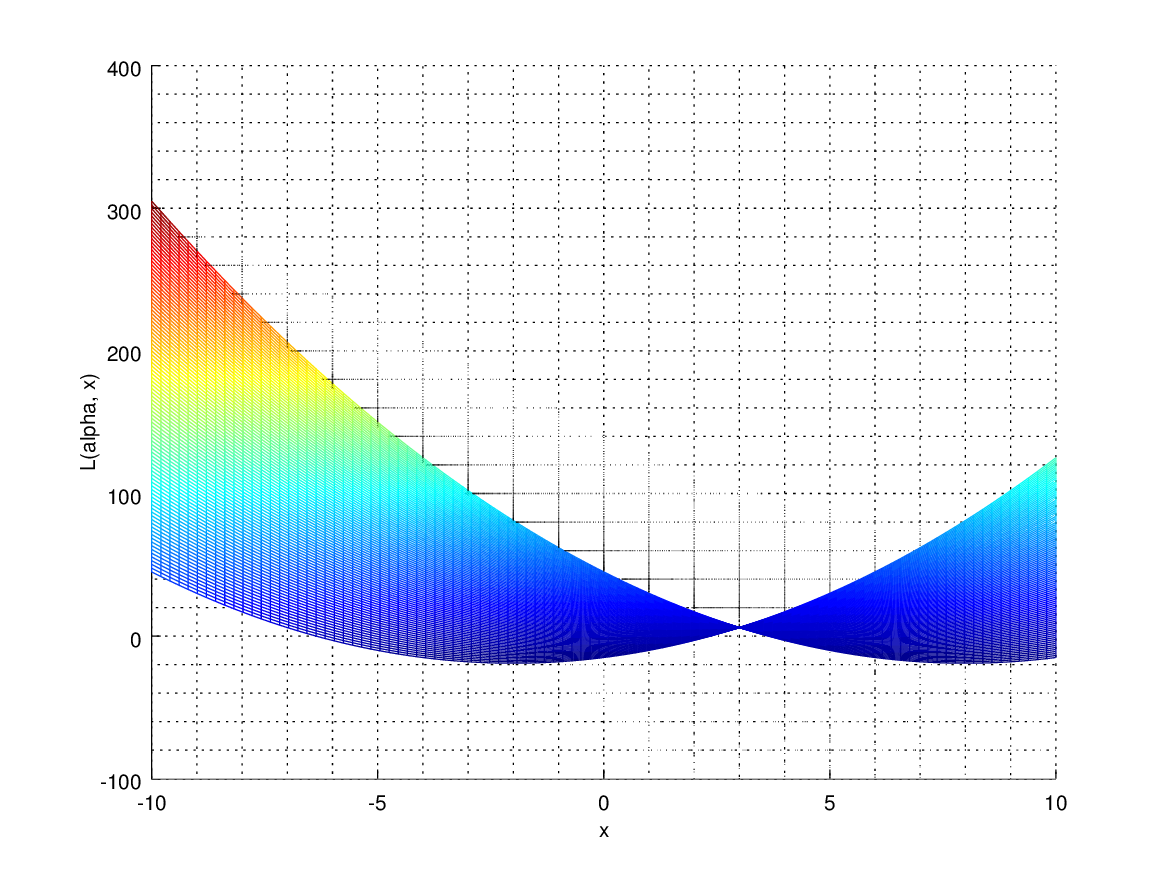
\includegraphics[width=\linewidth]{L_x.png}
  \caption{global minima ($x$)}\label{fig:awesome_image1}
\endminipage\hfill
\minipage{0.32\textwidth}
  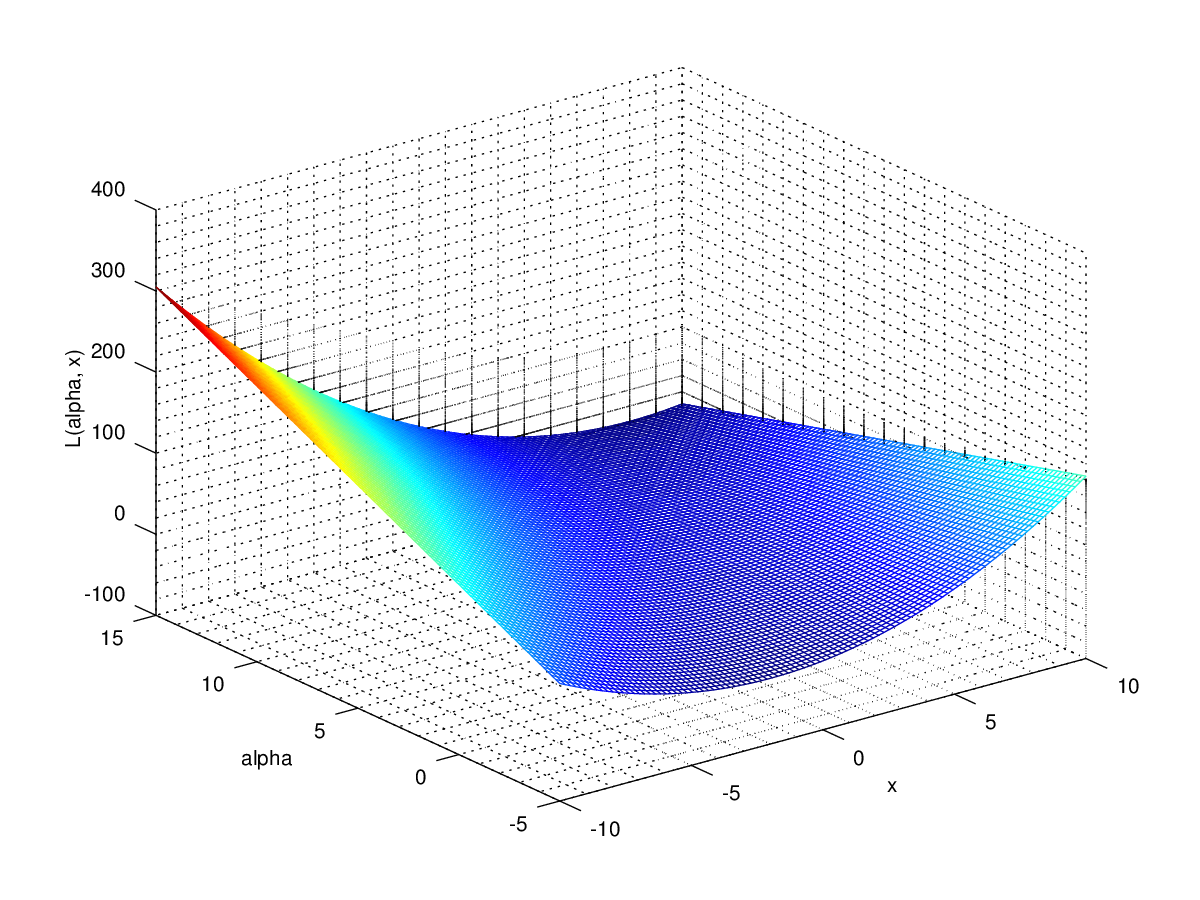
\includegraphics[width=\linewidth]{surface.png}
  \caption{Solution space}\label{fig:awesome_image2}
\endminipage\hfill
\minipage{0.32\textwidth}%
  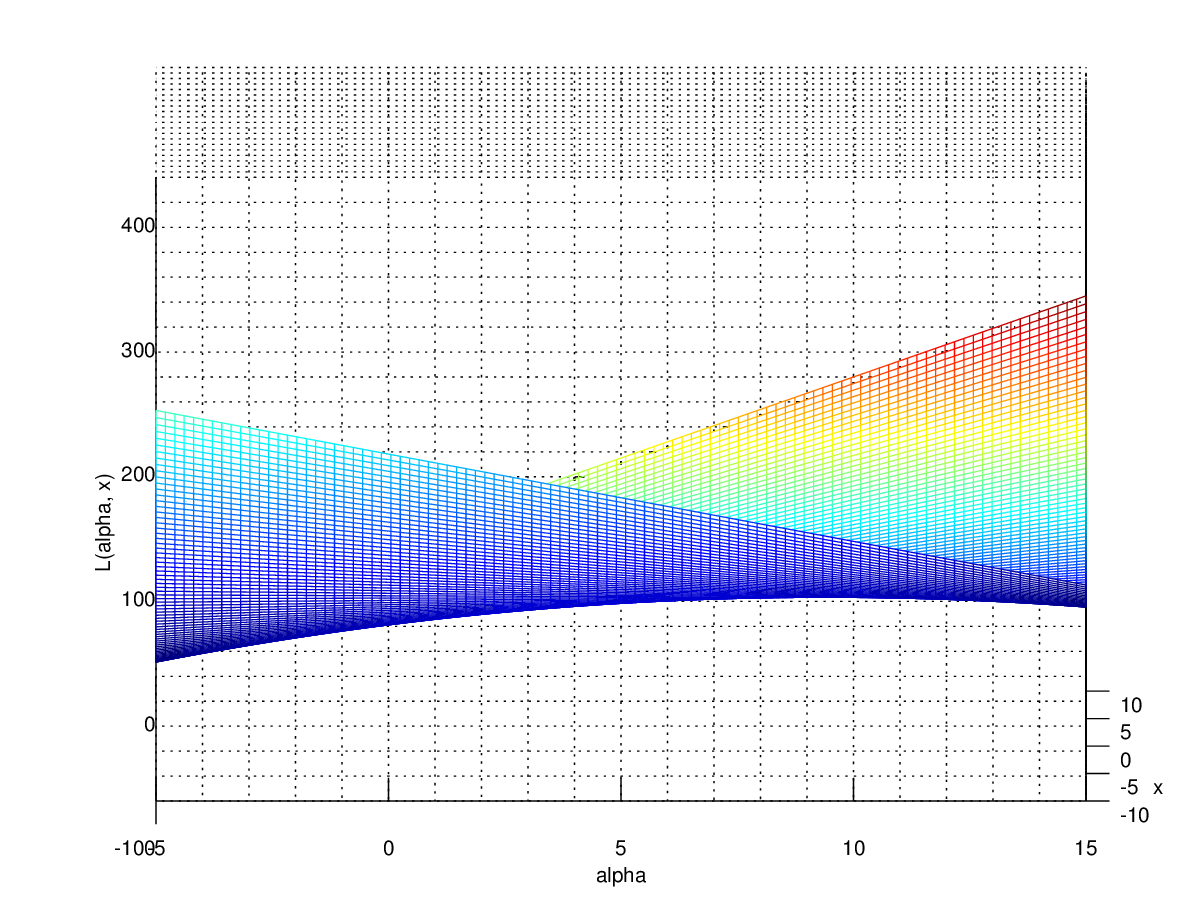
\includegraphics[width=\linewidth]{L_alpha.png}
  \caption{global maxima ($\alpha$) }\label{fig:awesome_image3}
\endminipage
\end{figure}
 

\section{Problem 7.3}

\begin{center}
$L(\bm{\alpha}, \mathbf{w}, b) = \frac{1}{2} \mathbf{w} \cdot \mathbf{w} - \smashoperator[r]{\sum_{i=1}^{\ell}} \alpha_i y_i \mathbf{w} \cdot \mathbf{x_i}
		 + b\smashoperator[r]{\sum_{i=1}^{\ell}} \alpha_i y_i + \smashoperator[r]{\sum_{i=1}^{\ell}} \alpha_i$
\end{center}


\def\A{
\begin{bmatrix}
    \pder{w_1} & \pder{w_2} & \cdots & \pder{w_n}
\end{bmatrix}}


Equation 7.41
$\\ \pder{L(\bm{\alpha}, \mathbf{w}, b)}{\mathbf{w}} = 	
\pder{\mathbf{w}}(\frac{1}{2} \mathbf{w} \cdot \mathbf{w}) - \pder{\mathbf{w}} (\smashoperator[r]{\sum_{i=1}^{\ell}} \alpha_i y_i \mathbf{w} \cdot \mathbf{x_i})
+ \cancel{\pder{\mathbf{w}}(b\smashoperator[r]{\sum_{i=1}^{\ell}} \alpha_i y_i)} + \cancel{\pder{\mathbf{w}}(\smashoperator[r]{\sum_{i=1}^{\ell}} \alpha_i)} = \frac{1}{2}\pder{\mathbf{w}} (\mathbf{w} \cdot \mathbf{w}) -  \smashoperator[r]{\sum_{i=1}^{\ell}} \alpha_i y_i \pder{\mathbf{w}}(\mathbf{w} \cdot \mathbf{x_i})$


$=\frac{1}{2} \A \mathbf{w} \cdot \mathbf{w} - \A \smashoperator[r]{\sum_{i=1}^{\ell}} \alpha_i y_i \mathbf{w} \cdot \mathbf{x_i}$


$=\frac{1}{2}\smashoperator[r]{\sum_{i=1}^{n}} \pder{w_i}(w_i^2)\hat{e_i} -  \smashoperator[r]{\sum_{i=1}^{\ell}} \left( \alpha_i y_i \smashoperator[r]{\sum_{k=1}^{n}} \pder{w_k}(w_k x_k) \hat{e_k} \right)$
$=\smashoperator[r]{\sum_{i=1}^{n}} w_i \hat{e_i} - \smashoperator[r]{\sum_{i=1}^{\ell}} \left( \alpha_i y_i \smashoperator[r]{\sum_{k=1}^{n}} x_k \hat{e_k} \right)\\ \\$ 

Since $\mathbf{w}$ and $\mathbf{x}$ are both in the same bector space ($\mathbf{R}^n$), they share the same standard basis vectors ($\hat{e_1}, \hat{e_2}, \dots, \hat{e_n}$)
this finally simplifies to $\mathbf{w} - \smashoperator[r]{\sum_{i=1}^{\ell}} \alpha_i y_i \mathbf{x_i}. \\$

Equation 7.43
$\\ \pder{L(\bm{\alpha}, \mathbf{w}, b)}{\mathbf{w}} =  \cancel{\pder{b} \left( \frac{1}{2} \mathbf{w} \cdot \mathbf{w} \right)} -  \cancel{\pder{b} \left(\smashoperator[r]{\sum_{i=1}^{\ell}} \alpha_i y_i \mathbf{w} \cdot \mathbf{x}\right)}
		 + \pder{b} \left( b\smashoperator[r]{\sum_{i=1}^{\ell}} \alpha_i y_i \right) +  \cancel{\pder{b} \left( \smashoperator[r]{\sum_{i=1}^{\ell}} \alpha_i\right) }
		 = \pder{b} \left( b\smashoperator[r]{\sum_{i=1}^{\ell}} \alpha_i y_i \right) = \smashoperator[r]{\sum_{i=1}^{\ell}} \alpha_i y_i$
		 
\pagebreak
\section{Problem 7.5}
\begin{center}
$L(\bm{\alpha}, \mathbf{w}, b) = \frac{1}{2} \mathbf{w} \cdot \mathbf{w} - \smashoperator[r]{\sum_{i=1}^{\ell}} \alpha_i y_i \mathbf{w} \cdot \mathbf{x}
		 + b\smashoperator[r]{\sum_{i=1}^{\ell}} \alpha_i y_i + \smashoperator[r]{\sum_{i=1}^{\ell}} \alpha_i$
\end{center}

By equation $7.43$, we have $\smashoperator[r]{\sum_{i=1}^{\ell}} \alpha_i y_i = 0$, and  $\bm{w^*} = \smashoperator[r]{\sum_{i=1}^{\ell}} \alpha_i y_i \mathbf{x_i}$
by equation $7.42.\\$

Now, consider the quantity $\bm{w^*}\bm{w^*}$:

\begin{center} \begin{math}		  
		   \bm{w^*}\bm{w^*} = \left( \smashoperator[r]{\sum_{i=1}^{\ell}} \alpha_i y_i \mathbf{x_i} \right) \cdot \left(\smashoperator[r]{\sum_{j=1}^{\ell}} \alpha_j y_j \mathbf{x_j} \right)
		   		      = \smashoperator[r]{\sum_{i=1}^{\ell}} \smashoperator[r]{\sum_{j=1}^{\ell}} \alpha_j \alpha_i y_j y_i \mathbf{x_j} \cdot \mathbf{x_i}
\end{math} \end{center}

And substitue these values into our laplacian:

\begin{center}  
	      $\pder{L(\bm{\alpha}, \mathbf{w}, b)}{\mathbf{w}}
	      = \frac{1}{2} \mathbf{w} \cdot \mathbf{w} - \smashoperator[r]{\sum_{i=1}^{\ell}} \alpha_i y_i \mathbf{w} \cdot \mathbf{x}
	      + \cancel{b\smashoperator[r]{\sum_{i=1}^{\ell}} \alpha_i y_i} + \smashoperator[r]{\sum_{i=1}^{\ell}} \alpha_i$
	      
	      $ = \frac{1}{2} \smashoperator[r]{\sum_{i=1}^{\ell}} \smashoperator[r]{\sum_{j=1}^{\ell}}  \alpha_j \alpha_i y_j y_i \mathbf{x_j} \cdot \mathbf{x_i}
	      - \smashoperator[r]{\sum_{i=1}^{\ell}} \alpha_i y_i \left( \smashoperator[r]{\sum_{j=1}^{\ell}} \alpha_j y_j \mathbf{x_j} \right) \cdot \mathbf{x_i}
	      + \smashoperator[r]{\sum_{i=1}^{\ell}} \alpha_i$
	      
	      $ = \frac{1}{2} \smashoperator[r]{\sum_{i=1}^{\ell}} \smashoperator[r]{\sum_{j=1}^{\ell}}  \alpha_j \alpha_i y_j y_i \mathbf{x_j} \cdot \mathbf{x_i}
	      - \smashoperator[r]{\sum_{i=1}^{\ell}} \smashoperator[r]{\sum_{j=1}^{\ell}}  \alpha_j \alpha_i y_j y_i \mathbf{x_j} \cdot \mathbf{x_i}
	      + \smashoperator[r]{\sum_{i=1}^{\ell}} \alpha_i$
	      
	      $ =\smashoperator[r]{\sum_{i=1}^{\ell}} \alpha_i - \frac{1}{2} \smashoperator[r]{\sum_{i=1}^{\ell}} \smashoperator[r]{\sum_{j=1}^{\ell}}  \alpha_j \alpha_i y_j y_i \mathbf{x_j} \cdot \mathbf{x_i} $
\end{center}


\end{document}

